\documentclass{article}
%
\usepackage[mathcal,mathbf]{euler}
%\usepackage{theorem,amsmath,enumerate,fancyhdr,amssymb,accents,amsfonts}
\usepackage{theorem,amsmath,enumerate,fancyhdr,amssymb,amsfonts}
\usepackage[pdftex]{graphics}

\usepackage{myDefs}

\begin{document}

\pagestyle{fancy}
\lhead{{\bf Assignment 1}
\\{\bf Author: }{Yuan Qu} } %insert lecture number
\rhead{{\bf Date: }01/31/2017} %enter lecture date NOT today's date

%
%%\oddsidemargin 0.0in 
%%\textwidth 6.25in 
%%\topmargin -0.25in 
%%\textheight 8.25in    

%% Write a quick short paragraph summarizing the topic covered in
%% the lecture here. You may use itemization or enumeration
\section*{Question 1}{
    Classify the following attributes as binary, discrete, or continuous. Also classify them as qualitative (nominal or ordinal) or quantitative (interval or ratio). Some cases may have more than one interpretation, so briefly indicate your reasoning if you think there may be some ambiguity.\\
    \textbf{Example:} Age in years. \textbf{Answer:} Discrete, quantitative, ratio
    \begin{enumerate}{
        \item Speed of a vehicle measured in mph.
        \item Altitude of a region.
        \item Intensity of rain as indicated using the values: no rain, intermittent rain, incessant rain. 
        \item Brightness as measured by a light meter.
        \item Barcode number printed on each item in a supermarket.
    }
    \end{enumerate}

    \paragraph{Answer: }{
        \begin{enumerate}{
            \item Continuous, quantitative, ratio.\\
            \item Continuous, quantitative, ratio.\\
            For some altitude graph, the altitude of a region is divided into colorful groups, it will be the qualitative ordinal data.
            \item Discrete, qualitative, ordinal.
            \item Continuous, quantitative, interval.\\
            Just consider it is same as Celsius, because light meter is not a precise and scientific measurement which has continuous range.
            \item Discrete, qualitative, nominal.
        }
        \end{enumerate}    
    }
}

\section*{Question 2}{
    The population for a clinical study has 500 Asian, 1000 Hispanic and 500 Native American people. What is good way of sampling this population to ensure that the distribution of various sub- populations is maintained if only 100 samples have to be chosen? Give the distribution of the various sub-populations in the final sample.

    \paragraph{Answer: }{
        In totality, the ratios of subpopulations are:

        \begin{center}{
            Asian : Hispanic : Native American = \(500:1000:500 = 1:2:1\)
        }
        \end{center}
        So, to ensure that the distribution of various subpopulations in sample:

        \(100\times(1+2+1)=25\)

        Asian: \(25\times1=25\)

        Hispanic: \(25\times2=50\)

        Native American: \(25\times1 = 50\)
    }
}

\section*{Question 3}{
    Justify your answers for the following:

    \begin{enumerate}{
        \item Is the Jaccard coefficient for two binary strings (i.e., string of 0s and 1s) always greater than or equal to their cosine similarity? 
        \item The cosine measure can range between $[-1,1]$. Give an example of a type of data for which the cosine measure will always be non-negative.
    }
    \end{enumerate}

    \paragraph{Answer 1: }{
        No, the cosine similarity is greater than or equal to the Jaccard coefficient.

        Consider two binary string $x$ and $y$. There are $k$ "1"s in $x$ and $m$ "1"s in $y$, and $r$ "1"s in \(x\wedge y\). 

        Obviously, \(k, m, r \geqslant 0\) and \(k\geqslant r, m\geqslant r\).

        According to the defination, 
        \begin{equation}
            cos(x,y) = \frac{x\cdot y}{\lvert\lvert x\rvert\rvert \cdot \lvert\lvert y\rvert\rvert}
        \end{equation}
        \begin{equation}
            \mathit{EJ}(x,y) = \frac{x\cdot y}{\lvert\lvert x\rvert\rvert^{2} \cdot \lvert\lvert y\rvert\rvert^{2} - x\cdot y}
        \end{equation}

        So, we have,
        \begin{center}{
            \(x\cdot y \geqslant 0, \lvert\lvert x\rvert\rvert = \sqrt{k},\) and \(\lvert\lvert y\rvert\rvert = \sqrt{m}\)
        }
        \end{center}

        Because the numerators of (1) and (2) are same and \(x\cdot y = r \geqslant 0\), so we only need to prove (3),
        \begin{equation}
             \lvert\lvert x\rvert\rvert^{2} \cdot \lvert\lvert y\rvert\rvert^{2} - x\cdot y \geqslant \lvert\lvert x\rvert\rvert \cdot \lvert\lvert y\rvert\rvert
        \end{equation}

        According to the defination, we can transform (3) to (4) and we only need to prove (4),
        \begin{equation}
            k + m - r \geqslant \sqrt{k\cdot m}
        \end{equation}

        Because \(k, m\geqslant 0\), \(k + m \geqslant 2 \sqrt{k\cdot m}\). So, 
        \begin{equation}
            k + m - r \geqslant 2\sqrt{k\cdot m} - r
        \end{equation}

        According to the defination, \(k\geqslant r, m\geqslant r\), so 
        \begin{equation}
            2\sqrt{k\cdot m} - r = \sqrt{k\cdot m} + (\sqrt{k\cdot m} - r) \geqslant \sqrt{k\cdot m}
        \end{equation}

        According to (5) and (6), the (4) is proved. So,
        \[cos(x,y) \geqslant \mathit{EJ}(x,y)\]
        The "greater than or equal to" could be "equal to" only if \(k = m = r\).
    }

    \paragraph{Answer 2: }{
        According to the defination,
        \[cos(x,y) = \frac{x\cdot y}{\lvert\lvert x\rvert\rvert \cdot \lvert\lvert y\rvert\rvert}\]
        
        So, to make cosine measure be non-negative is equal to make \(x\cdot y\) non-negative. 

        There are two situations:
        \begin{enumerate}{
            \item When vectors are all in non-negetive numbers(or all in negative) the cosine measure will always be non-negative.\\
            \textit{e.g.} the ratings range from 1 to 10 or a whatever postive integer, the stars(can be regard as range 1-5) and the number of transactions.
            \item The data is highly centralized and far from the origin. In geometry, the cosine measure can be explain to the angle between vectors, so small angle(less than \(\pi/2\)) means non-negative cosine. If the data is highly centralized, the angles will be very small and the cosine will be non-negative.\\
            \textit{e.g.} all the types of data could be in this situation if an improper model is chosen.
        }
        \end{enumerate} 
    }
}

\section*{Question 4}{
    The similarity between two undirected graphs G1 and G2 that have the same n vertices can be defined using:
    \[\mathit{S(G_1, G_2)}=\frac{\sum_{i}{}min(deg(\mathit{v_i} \in \mathit{G_1}), deg(\mathit{v_i} \in \mathit{G_2}))}{2 \times max(\lvert\mathit{G_1}\rvert,\lvert\mathit{G_2}\rvert)}\]
    where \(\mathit{deg(v \in G)}\) indicates the degree of a vertex $v$ in graph $G$ and $|G|$ indicates the number of edges in G.

    If \(\mathit{S(G_1, G_2)}\) = 1, are the two graphs equivalent? Provide an example to justify your answer.

    \paragraph{Answer: }{
        No.

        If two graphs are quivalent, obviously, 
        \(\mathit{S(G_1, G_2)}\) = 1. But for the converse situation, it is easy to built a counter-example like that:

        \begin{center}{
            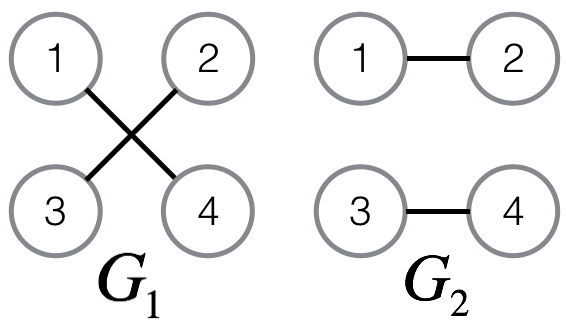
\includegraphics{graph.png}
        }
        \end{center}
        
        In this case, 
        \[\mathit{S(G_1, G_2)}=\frac{\sum_{i=1}^{4}min(deg(\mathit{v_i} \in \mathit{G_1}), deg(\mathit{v_i} \in \mathit{G_2}))}{2 \times max(\lvert\mathit{G_1}\rvert,\lvert\mathit{G_2}\rvert)}=\frac{1 + 1 + 1 + 1}{2 \times 2}=1\]
        but \(\mathit{G_1}\) and \(\mathit{G_2}\) are different.
    }
}

\section*{Question 5}{
    For every item \(\mathit{i}\) in a grocery store, a set \(\mathit{s_i}\) is used to represent the IDs of transactions in which \(\mathit{i}\) is purchased. Assume that the data set to be analyzed contains hundreds of thousands of such transactions.
    \begin{enumerate}{
        \item In order to analyze the proximity between any two of these sets \(\mathit{s_i}\) and \(\mathit{s_j}\), which measure, Jaccard or Hamming, would be more appropriate and why ?
        \item In order to analyze the proximity between any two of these sets \(\mathit{s_i}\) and \(\mathit{s_j}\) for items \(\mathit{i}\) and \(\mathit{j}\) that are often brought together (example: milk, bread), which measure, Jaccard or Hamming, would be more appropriate and why ?
    }
    \end{enumerate}

    \paragraph{Answer: }{
        Assumed that the number of total transactions is \(\mathit{n}\) and for the item \(\mathit{r}\), the set \(\mathit{s_r}={id_1, id_4, ..., id_{n-2}, id_n}\). Obviously, each two sets may not have same length(same times be purchased).

        To analyze the proximity between any of two sets, we have to standardize the sets \(\mathit{s_i}\) into constant length $n$. The standardization is to change IDs sets to binary set in \(\mathit{n}\) digit, in which the \(\mathit{id_i}\) are transformed to the "1" at \(\mathit{i}\) digit, for instance, 
        \[\mathit{s_r}=10010...0101\]

        Aussumed that \(\lvert\mathit{s_i}\rvert=k, \lvert\mathit{s_j}\rvert=m\) and \(\lvert\mathit{s_i}\cap\mathit{s_j}\rvert=l\), according to the defination, we have:

        \[Jaccard: \mathit{J}=\frac{l}{k+m-l} \text{, which measure similarity.}\]

        and

        \[Hamming: \mathit{H}=k+m-2\times l \text{, which measure distinction.}\]

        In the (1) situation, Jaccard measure would be more appropriate. In this case, the goal is to find the similar binary vectors, so we choose similarity measurement here.

        In the (2) situation, Hamming measure would be more appropriate. In this case, the goal is to distinct the level or degree of similarity, so we choose distinction measurement here.
    } 
}

\section*{Question 6}{
    For the data set described below, give an example of the types of data mining questions that can be asked (one for each classification, clustering, association rule mining, and anomaly detection task) and the description of the data matrix (what are the rows and columns). If necessary, briefly explain the features that need to be constructed. Note that, depending on your data-mining question, the row and column definitions may be different.

    Example data: a collection of Web pages.

    A clinical dataset containing various measures like temperature, blood pressure, blood glucose and heart rate for each patient during every visit, along with the diagnosis information.

    \paragraph{Answer: }{
        \begin{itemize}{
            \item DM Task: Classification of patients\\
            Question: What type of patient?\\
            Row: A record of a patient.\\
            Column: temperature, blood pressure, blood glucose, heart rate and labels.\\
            Label: Fever(high temperature, others normal), hypertension(high blood pressure), hypotension(low blood pressure), diabetes(high blood glucose), coronary disease(high blood pressure, high heart rate), healthy(all normal).\\
            Rules: Use these labels to classify all the patients.
            \item DM Task: Clustering of patients\\
            Question: What are the patients with similar diseases?\\
            Row: A record of a patient.\\
            Column: temperature, blood pressure, blood glucose and heart rate.\\
            Rules: Use clustering method to cluster data, find the group that the points are centralized.
            \item DM Task: Association rule mining\\
            Question: What are the symptoms that appear together frequently?\\
            Row: A record of a patient.\\
            Column: temperature, blood pressure, blood glucose and heart rate.\\
            Rules: For instance, most people with coronary disease have high blood pressure, high blood glucose and high heart rate as the symptoms, and most people with high blood glucose will also have high blood pressure.
            \item Anomaly detection\\
            Question: Is it a patient need first-aid?\\
            Row: A record of a patient.\\
            Column: temperature, is temperature critical(a boolean value), blood pressure, is blood pressure critical(a boolean value), blood glucose, is blood glucose critical(a boolean value), heart rate and is heart rate critical(a boolean value).\\
            Rules: According to the training set, we can get the distribution or clustering margin of each feature and set a critical value for each feature. When the new data come in, as the test set, judge the features are critical or not, if critical, set the record as anomaly.
        }
        \end{itemize}
    }
}



%\begin{enumerate}
%\item 
%\item
%etc
%\end{enumerate}


%\subsection{ }
%\subsubsection{ }

%\begin{center}
%\includegraphics[scale=0.5]{filename.pdf}
%\end{center}

\end{document}
